\documentclass[a4paper]{scrartcl}
\usepackage[cm]{fullpage}
\usepackage{amsmath, amssymb, esint}
\usepackage{siunitx}
\usepackage{tikz, pgfplots}

\begin{document}

\title{PHYS2114: Assignment 2}
\author{ \\ \\ }
\date{2016-10-25}
\maketitle

\section{Design a broadband anti-reflection coating for use on a material with refractive index \(n_s = 2.8\) exposed to air (\(n_0 = 1.0\)) while having a maximum transmittance at \(\lambda_0 = \SI{750}{\nano\metre}\) and at least three layers.}

While a continuously graded index from 1.0 to 2.8 would be optimal, it is unrealistic to construct. Instead, let us limit possible layer refractive indices to between 1.3 and 2.8 with a maximum precision of 0.05. Layers will also be limited to a thickness precision of \SI{1}{\nano\metre}. For simplicity, dispersion and absorption effects are ignored, and only normal incidence will be considered.

\subsection{Calculate the refractive indices and thicknesses of the coating layers.}
\begin{table}
    \centering
    \begin{tabular}{c | c | c}
        Layer & Index & Thickness (\si{\nano\metre}) \\
        \hline
        0 (Air) & 1.00 & \(\infty\) \\
        1 & 1.30 & 131 \\
        2 & 1.70 & 100 \\
        3 & 1.85 & 92 \\
        4 & 2.05 & 83 \\
        5 & 2.30 & 74 \\
        6 & 2.55 & 67 \\
        S (Substrate) & 2.80 & \(\infty\)
    \end{tabular}
    \caption{Layer specifications}
    \label{tab:layers}
\end{table}

Table \ref{tab:layers} shows the details. Actually finding materials of the specified indices will be difficult, but this can be resolved by restricting the indices through the use of techniques such as Southwell's flip-flop technique --- but those are outside of the scope of this assignment.

The indices were found by first considering our minimum index of 1.3. Obviously, this will be the first layer, since any higher will produce an even stronger reflection. The next layer is merely applying the same ratio between the air and first layer to the first layer to minimise the effect of the large jump in refractive index of the first layer --- it optimally destructively interferes with the reflections produced by the first layer around our target wavelength of \(\lambda_0\). The remaining indices are just a constant ratios of 1.106 up to \(n_s\).

6 layers were chosen because it produced the best result in numerical simulations. Unfortunately, this produces 7 boundaries --- an odd number, which means that we cannot perfectly destructively interfere our target wavelength with quarter wave layers. Fortunately, two smaller minima a little away from our target wavelength replaced the perfect minima on the addition of the 6th layer. By adjusting the layer thicknesses to be quarter wave layers for a wavelength of \SI{680}{\nano\metre}, one of the minima was moved to \(\lambda_0 = \SI{750}{\nano\metre}\).

Calculating the thickness for a quarter wave layer is trivial:
\[d = \frac{\lambda}{4 n}\]
where \(n\) is the refractive index of the medium.

\subsection{Write down the matrix expression used to determine the reflectance coefficient \(r\) from this structure.}
Let us first consider what happens at a boundary. Let \(a\) be the source layer number and \(b\) be the destination. Our Fresnel coefficients and transfer matrix will then be:
\begin{align*}
    r_{a \rightarrow b} &= \frac{n_a - n_b}{n_a + n_b} \\
    t_{a \rightarrow b} &= \frac{2 n_a}{n_a + n_b} \\
    \mathbf{D}_{a \rightarrow b} &= \frac{1}{t_{a \rightarrow b}} \begin{pmatrix}
        1 & r_{a \rightarrow b} \\
        r_{a \rightarrow b} & 1
    \end{pmatrix}
\end{align*}

This relates the incident wave amplitude to its resultant waves at the boundary, where \(E\) denotes a left travelling wave and \(E'\) a right:
\[\begin{pmatrix}E_a \\ E_a'\end{pmatrix} = \mathbf{D}_{a \rightarrow b} \begin{pmatrix}E_b \\ E_b'\end{pmatrix}\]

Since the layers have finite thickness \(d_m\), there will also be a phase shift \(\phi_m\) as the wave travels through them. This can be represented as another transfer matrix \(\mathbf{P}_m\), where \(m\) is the medium number:
\begin{align*}
    \phi_m &= 2 \pi \frac{n_m d_m}{\lambda} \\
    \mathbf{P}_m &= \begin{pmatrix}
        e^{-i \phi_m} & 0 \\
        0 & e^{i \phi_m}
    \end{pmatrix}
\end{align*}

These can be combined together to model the entire wave propagation:
\[\begin{pmatrix}E_0 \\ E_0'\end{pmatrix} = \left(\prod_{i = 0}^N \mathbf{D}_{i \rightarrow i + 1} \mathbf{P}_{i + 1}\right) \mathbf{D}_{N \rightarrow S} \begin{pmatrix}E_S \\ E_S'\end{pmatrix}\]
where \(N\) is the total number of layers.

Since the reflectance coefficient is simply what proportion of amplitude is the reflected wave of the incidence:
\[r = \frac{E_0'}{E_0}\]
and we assume any wave that has entered the substrate travels to infinite (\(E_s' = 0\)), we can set \(E_S\) to any arbitrary convenient non-zero value such as 1:
\[\begin{pmatrix}E_0 \\ E_0'\end{pmatrix} = \left(\prod_{i = 0}^N \mathbf{D}_{i \rightarrow i + 1} \mathbf{P}_{i + 1}\right) \mathbf{D}_{N \rightarrow S} \begin{pmatrix}1 \\ 0\end{pmatrix}\]

\subsection{Plot the reflectivity \(R = |r|^2\) between \SI{400}{\nano\metre} and \SI{1100}{\nano\metre}, and mark the important features.}
\begin{figure}
    \centering
    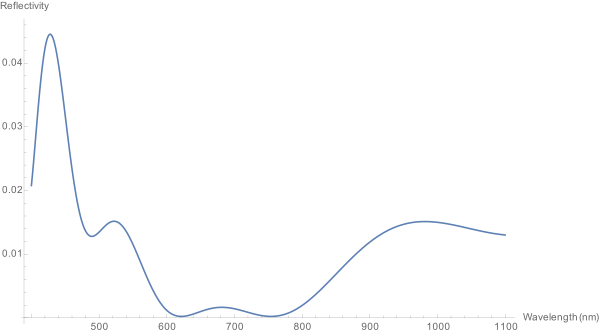
\includegraphics[width = 18cm]{reflectivity-lin.png}
    \caption{Reflectivity of the coating}
    \label{fig:reflectivity-lin}
\end{figure}
\begin{figure}
    \centering
    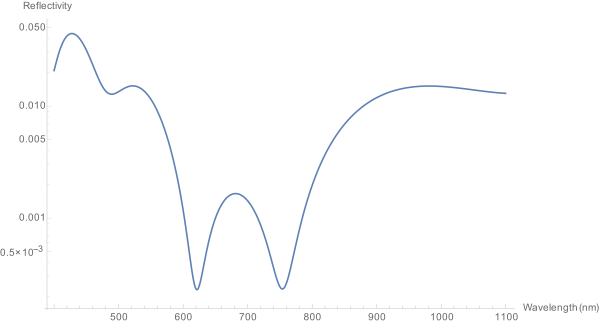
\includegraphics[width = 18cm]{reflectivity-log.png}
    \caption{Same as Figure \ref{fig:reflectivity-lin}, but on a logarithmic scale}
    \label{fig:reflectivity-log}
\end{figure}

The reflectivity is plotted in Figures \ref{fig:reflectivity-lin} and \ref{fig:reflectivity-log}. Markers 1 and 2 denote the ``two smaller minima'' mentioned in section 1.1 at \SI{750}{\nano\metre} and \SI{620}{\nano\metre} with reflectivities of \SI{0.023}{\percent}. Marker 3 shows where the ``perfect minima'' (= 0 reflectivity) at \SI{680}{\nano\metre} would have been if an odd number of layers were used, but now is a local maxima of \SI{0.17}{\percent}. Marker 4 shows the largest maxima in the plot at \SI{425}{\nano\metre} of \SI{4.5}{\percent}.

In general, the minima and maxima occur due to the reflections from each layer phasing in and out from each other. Minima simply are where they were more out of phase (destructive) than the maxima, where there were more in phase (constructive).

\subsection{Assuming the substrate is being illuminated at all wavelengths between \SI{400}{\nano\metre} and \SI{1100}{\nano\metre} equally, calculate the proportion of light lost by reflection on both the coated version and uncoated, and compare.}
This is simply an averaging operation of \(R\) over the wavelength range:
\[\frac{1}{\lambda_2 - \lambda_1} \int_{\lambda_1}^{\lambda_2} R \:\mathrm{d \lambda}\]
where \(\lambda_1 = \SI{400}{\nano\metre}\) and \(\lambda_2 = \SI{1100}{\nano\metre}\)

For the coated substrate, this turns out to be \SI{1.06}{\percent} loss, while the uncoated has \SI{22.4}{\percent}. This is a ratio of:
\[\frac{\SI{1.06}{\percent}}{\SI{22.4}{\percent}} \approx 0.0474 \approx \SI{-26.5}{\decibel} \approx \frac{1}{21.1}\]

In other words, the coating has reduced reflection attenuation by \SI{26.5}{\decibel}. In layman terms, that is an ``improvement'' of \(21\times\).

\end{document}